% 本章节主要介绍有关操作系统的内容
\section{操作系统——基于Linux}
本章节是根据 向勇和陈渝老师的操作系统公开课\cite{Operating_System_Risc-V},还有 \cite{操作系统先修课} \cite{从按下电源开始的一场接力赛} \cite{完善Kernel——输入输出管理} \cite{完善Kernel——内存管理} \cite{完善Kernel——进程管理} \cite{完善Kernel——文件管理} \cite{完善Kernel——用户接口实现交互} \cite{用软件工程的方式完成操作系统课设——制作一个操作系统} 改编完成的。
\subsection{从OS角度看系统结构}
为什么要使用计算机,在以前没有计算机的时候,人们依旧可以每天正常生活,那计算机存在的意义是是什么?我认为应该是高效,他解放了生产力,他比人类手工更适合信息的处理。

那当年的计算机科学家为什么要提出体系结构,可能是想让计算机变得跟高效,操作系统就是一种让计算机变得跟高效的一种技术,因为有了操作系统就可以在一个CPU上运行多了程序(一般我们称之为\textbf{进程}),多了进程之前运行还要保证相互之间没有影响,这就需要进行隔离,而如何进行隔离有时系统结构给予的支持(主要是虚拟存储,中断技术)。

\begin{figure}[htbp]
  \centering %居中显示
  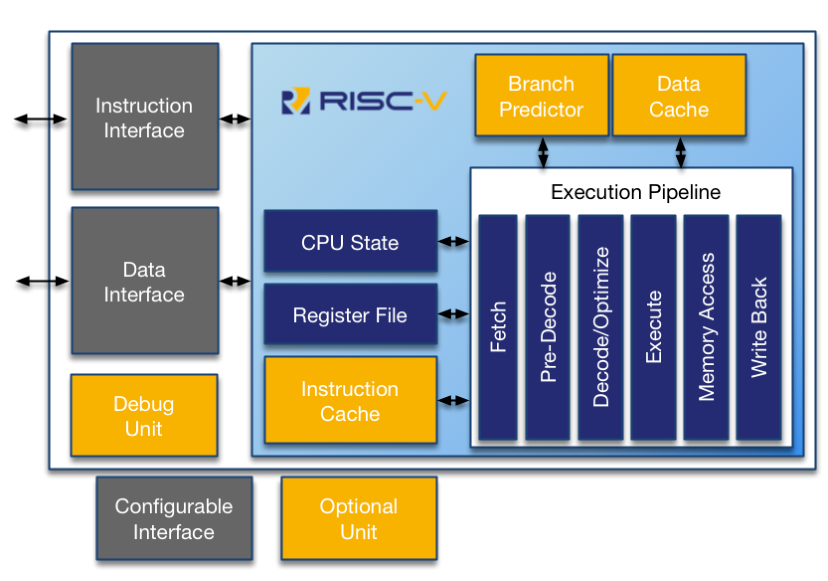
\includegraphics[width=0.6 \textwidth]{figs/OS/RISC_V.png}
  \caption{RISC-V的CPU结构}
  \label{fig:RISC_V_CPU} %设置图形引用名称
\end{figure}

图\ref{fig:RISC_V_CPU}是RISC-V的CPU结构,这就是CPU的典型结构。我们举例说明一下,来体现一下操作系统是如何与体系结构之间结合在一起的,如图\ref{fig:MMU_TLB_page}所示,是基于虚拟存储的地址空间隔离,首先是经典的5级流水线,取值和访存阶段是需要使用TLB的,但是也存在页表讲虚拟地址转化为实际的物理地址的过程,完美配合,这样既保证了操作系统的安全性,也提升了计算机整体的性能。

\begin{figure}[htbp]
  \centering %居中显示
  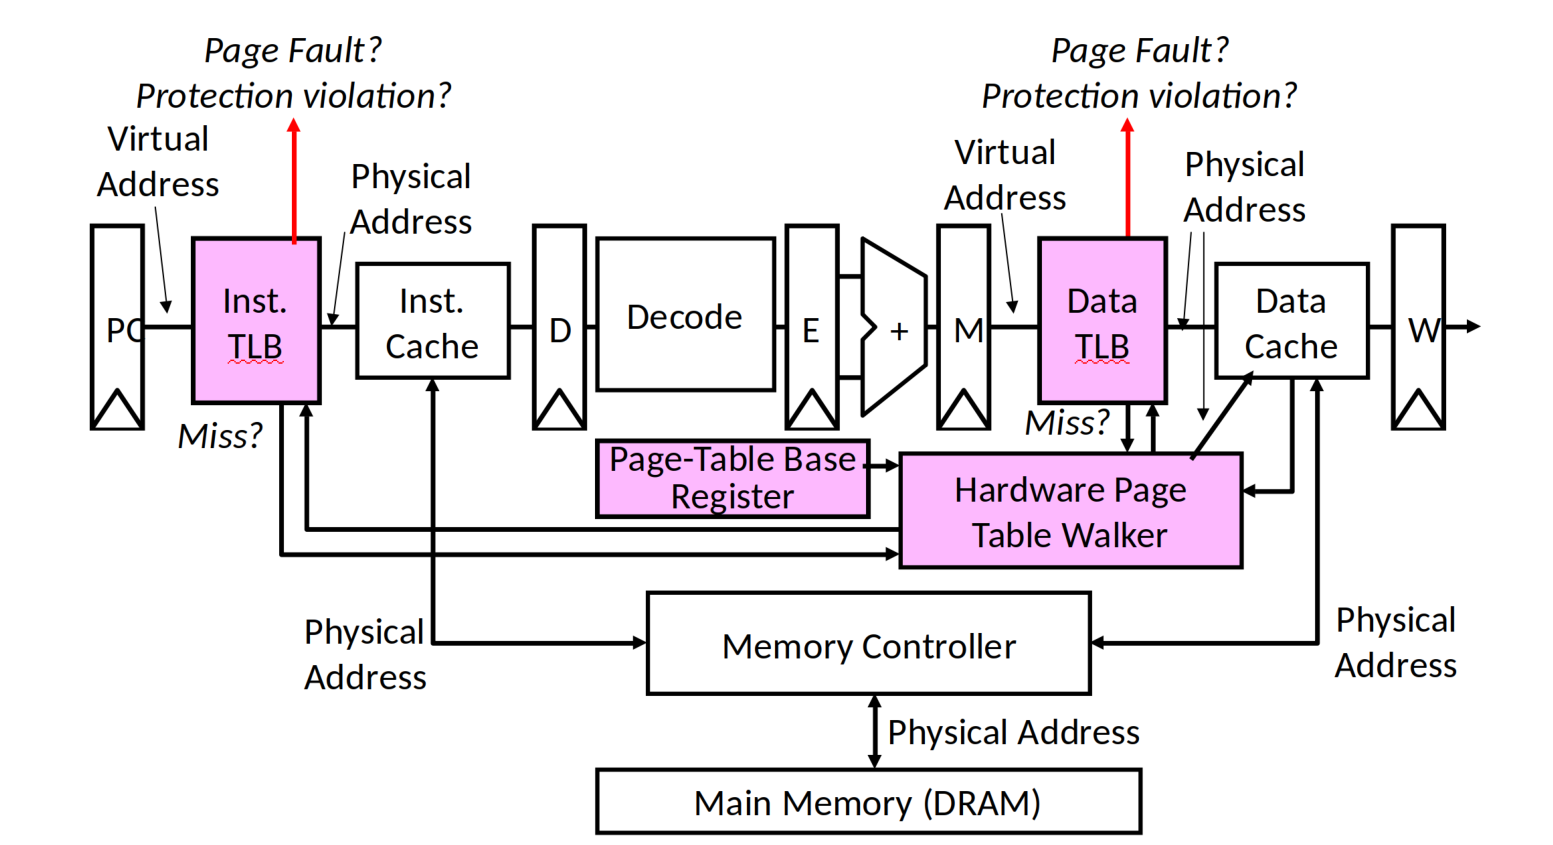
\includegraphics[width=0.9 \textwidth]{figs/OS/MMU_TLB_page.png}
  \caption{带MMU/TLB的操作系统使用页表}
  \label{fig:MMU_TLB_page} %设置图形引用名称
\end{figure}

还有就是特权模式,现在很多CPU硬件支持不同的特权模式,常见的是Kernel Mode与User Mode,两者之间的转换依靠“中断”,CPU在每一条指令的间隙都会检查是否有中断请求,如果有立即停下来正在做的事情,处理中断请求。一般有一个中断处理程序,用来相应中断,I/O设备通过向处理器芯片的一个引脚法请求,并将异常信号发送到系统总线上,触发中断;处理器在指令间隙的时候(一般系统都是分时操作系统,有一个Timer可以稳定且定时产生中断,这样可以防止应用程序占着CPU不放),会从系统总线读取异常号,发现有中断需要处理,立即保存现场,切换到Kernel Mode;调用中断处理程序,当中断处理程序完成后,恢复现场,执行本该执行的下一条指令。

\subsection{从OS角度看RISC-V的CPU}
\subsubsection{RISC-V与操作系统的关系}
如图\ref{fig:计算机系统的抽象层次}所示,RISC-V是一种指令集体系结构(ISA),ISA作为软硬件接口,操作系统是第一个与其接触的软件,具体参见\cite{CS61c},如图\ref{fig:软硬件接口}

\begin{figure}[htbp]
  \centering %居中显示
  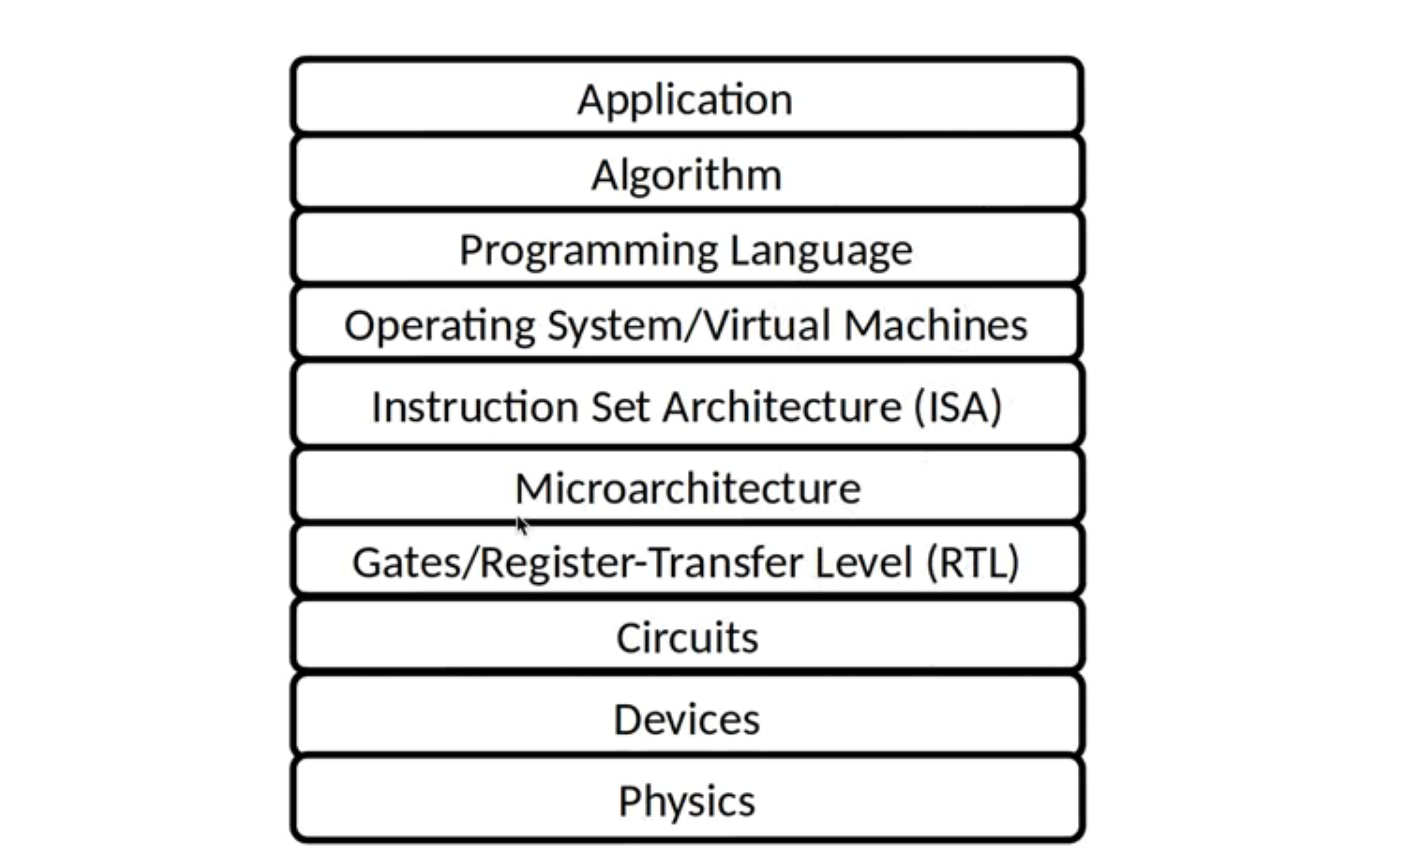
\includegraphics[width=0.9 \textwidth]{figs/OS/计算机系统的抽象层次.png}
  \caption{计算机系统的抽象层次}
  \label{fig:计算机系统的抽象层次} %设置图形引用名称
\end{figure}

\begin{figure}[htbp]
  \centering %居中显示
  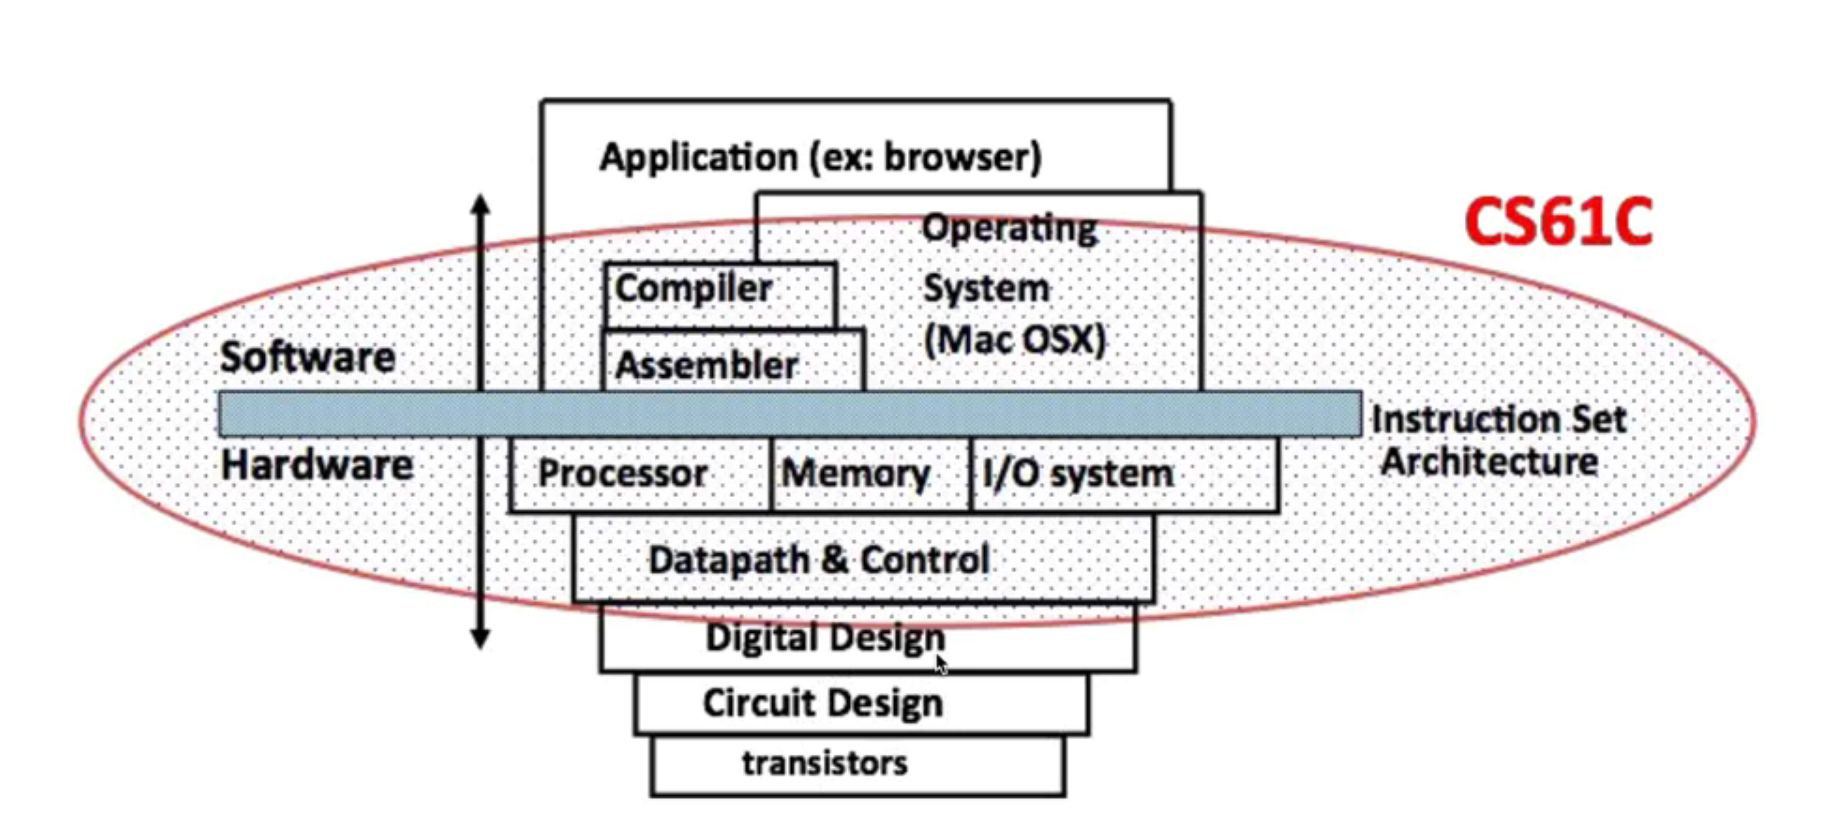
\includegraphics[width=0.9 \textwidth]{figs/OS/软硬件接口.png}
  \caption{软硬件接口}
  \label{fig:软硬件接口} %设置图形引用名称
\end{figure}

\subsubsection{RISC-V CPU与其他CPU有什么不一样}
RISC-V不像Intel和ARM没有太多历史包袱,

在特权架构方面,RISC-V与x86都有四种模式,U:User、S:Supervisor、H:Hypervisor、M:Machine

RISC-V设置CSR(控制状态寄存器)实现隔离,防止其他应用访问设备和敏感的CPU寄存器(eg:地址空间寄存器)





